\documentclass[11pt,aspectratio=169,t]{beamer}

\usepackage[T1]{fontenc}
\usepackage{lmodern}
\usepackage{amsmath,amssymb,mathtools}
\usepackage{booktabs}
\usepackage{graphicx}
\usepackage{tikz}
\usetikzlibrary{arrows.meta,positioning,shapes.geometric,calc,backgrounds,fit}
\usepackage[mode=tex]{standalone}

% Clean, spacious academic palette
\definecolor{sknavy}{HTML}{0F2952}
\definecolor{skslate}{HTML}{334155}
\definecolor{skmuted}{HTML}{64748B}
\definecolor{skteal}{HTML}{0F766E}
\definecolor{skcrimson}{HTML}{B91C1C}
\definecolor{skamber}{HTML}{B45309}
\definecolor{skbg}{HTML}{F8FAFC}
\definecolor{skcard}{HTML}{F1F5F9}
\definecolor{skline}{HTML}{CBD5E1}
\definecolor{skmint}{HTML}{ECFDF5}
\definecolor{skrose}{HTML}{FEF2F2}
\definecolor{skgold}{HTML}{FFFBEB}

\usetheme{default}
\usefonttheme{professionalfonts}
\setbeamertemplate{navigation symbols}{}
\setbeamersize{text margin left=8mm,text margin right=8mm}

\setbeamercolor{normal text}{fg=skslate,bg=white}
\setbeamercolor{structure}{fg=sknavy}
\setbeamercolor{frametitle}{fg=sknavy,bg=white}
\setbeamercolor{framesubtitle}{fg=skmuted}
\setbeamercolor{itemize item}{fg=sknavy}
\setbeamercolor{itemize subitem}{fg=skteal}

\setbeamerfont{frametitle}{size=\Large,series=\bfseries}
\setbeamerfont{framesubtitle}{size=\small,series=\mdseries}

\setbeamertemplate{itemize item}{\raisebox{0.12ex}{\tikz\fill[sknavy] (0,0) circle (1.6pt);}}
\setbeamertemplate{itemize subitem}{\raisebox{0.12ex}{\tikz\fill[skteal] (0,0) circle (1.3pt);}}

\setbeamertemplate{frametitle}{%
  \vspace{3.5mm}%
  \insertframetitle\par%
  \ifx\insertframesubtitle\@empty\else%
    \vspace{0.6mm}{\usebeamerfont{framesubtitle}\usebeamercolor[fg]{framesubtitle}\insertframesubtitle\par}%
  \fi%
  \vspace{1.2mm}%
}

\setbeamertemplate{footline}{%
  \leavevmode%
  \hbox{%
    \begin{beamercolorbox}[wd=.75\paperwidth,ht=2.6ex,dp=1.2ex,leftskip=8mm]{fg=skmuted}%
      \scriptsize Knotted Surfaces in $\mathbb{R}^4$ ($\operatorname{ch} \le 12$)%
    \end{beamercolorbox}%
    \begin{beamercolorbox}[wd=.25\paperwidth,ht=2.6ex,dp=1.2ex,rightskip=8mm,right]{fg=skmuted}%
      \scriptsize \insertframenumber{} / \inserttotalframenumber%
    \end{beamercolorbox}%
  }%
  \vskip2pt%
}

\newcommand{\ch}{\operatorname{ch}}
\newcommand{\defi}{\operatorname{def}}
\newcommand{\RP}{\mathbb{RP}^2}
\newcommand{\Z}{\mathbb{Z}}
\newcommand{\SL}{\mathrm{SL}}

\newcommand{\badge}[2]{%
  \tikz[baseline=(b.base)]\node[fill=#1!14,draw=#1!65,text=#1!95!black,rounded corners=2.5pt,inner xsep=4.5pt,inner ysep=1.5pt,font=\scriptsize\bfseries] (b) {#2};%
}

\newcommand{\minidiag}[3]{%
  \begin{minipage}[t]{#1}\centering
    \includestandalone[width=0.92\linewidth,height=1.75cm,keepaspectratio]{#2}\\[1pt]
    {\tiny\bfseries\color{sknavy} #3}
  \end{minipage}%
}

\begin{document}

% ==================================================================
% SLIDE 1: TITLE SLIDE
% ==================================================================
\begin{frame}[plain]
  \vspace*{6mm}
  \begin{center}
    {\huge\bfseries\color{sknavy} Knotted Surfaces in $\mathbb{R}^4$}\\[2.5mm]
    {\large\color{skslate} An Exhaustive Machine Census Through $\ch \le 12$}\\[6mm]

    \begin{tikzpicture}[
      card/.style={draw=skline, fill=skbg, rounded corners=6pt, inner sep=4pt, minimum width=2.4cm, minimum height=2.8cm}
    ]
      \node[card] (c1) at (0,0) {
        \begin{minipage}{2.15cm}\centering
          \includestandalone[height=1.9cm,keepaspectratio]{../pics/tikz/8_1}\\[2pt]
          {\scriptsize\bfseries\color{sknavy} $8_1$}\;{\scriptsize\color{skmuted} (spun $3_1$)}
        \end{minipage}
      };
      \node[card] (c2) at (2.75,0) {
        \begin{minipage}{2.15cm}\centering
          \includestandalone[height=1.9cm,keepaspectratio]{../pics/tikz/10_2}\\[2pt]
          {\scriptsize\bfseries\color{sknavy} $10_2$}\;{\scriptsize\color{skmuted} ($2$-twist $3_1$)}
        \end{minipage}
      };
      \node[card] (c3) at (5.50,0) {
        \begin{minipage}{2.15cm}\centering
          \includestandalone[height=1.9cm,keepaspectratio]{../pics/tikz/11_1_sup_m2}\\[2pt]
          {\scriptsize\bfseries\color{sknavy} $11_1^{-2}$}\;{\scriptsize\color{skmuted} ($2O$ $K^2$)}
        \end{minipage}
      };
      \node[card] (c4) at (8.25,0) {
        \begin{minipage}{2.15cm}\centering
          \includestandalone[height=1.9cm,keepaspectratio]{../pics/tikz/11_2}\\[2pt]
          {\scriptsize\bfseries\color{sknavy} $11_2$}\;{\scriptsize\color{skmuted} (ribbon $S^2$)}
        \end{minipage}
      };
      \node[card] (c5) at (11.00,0) {
        \begin{minipage}{2.15cm}\centering
          \includestandalone[height=1.9cm,keepaspectratio]{figs/12_10}\\[2pt]
          {\scriptsize\bfseries\color{sknavy} $12_{10}$}\;{\scriptsize\color{skmuted} (CS $S^2$)}
        \end{minipage}
      };
    \end{tikzpicture}

    \vspace{5.5mm}
    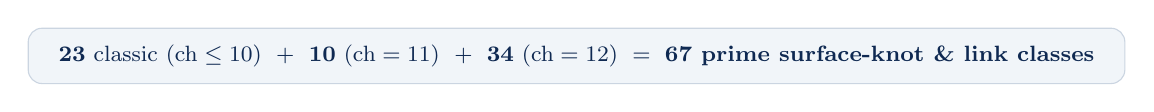
\begin{tikzpicture}
      \node[fill=skcard, draw=skline, rounded corners=5pt, inner xsep=11pt, inner ysep=6pt, font=\footnotesize\color{sknavy}] {
        \textbf{23} classic ($\ch \le 10$) $\;+\;$ \textbf{10} ($\ch = 11$) $\;+\;$ \textbf{34} ($\ch = 12$) $\;=\;$ \textbf{67 prime surface-knot \& link classes}
      };
    \end{tikzpicture}
  \end{center}
\end{frame}

% ==================================================================
% SLIDE 2: WHY TABULATE SURFACES IN R^4? (1D VS 2D)
% ==================================================================
\begin{frame}{Why Tabulate Surfaces in $\mathbb{R}^4$?}
  \framesubtitle{Classical knot tables reach $\ge 16$ crossings; the 1994 surface-knot table stopped at $10$ vertices ($23$ surfaces)}

  \begin{columns}[c,totalwidth=\textwidth]
    \begin{column}{0.43\textwidth}
      \begin{tikzpicture}
        \node[draw=skline, fill=skbg, rounded corners=6pt, inner sep=8pt, text width=0.92\linewidth] {
          {\bfseries\color{sknavy} Classical Knots: $S^1 \hookrightarrow \mathbb{R}^3$}\\[6pt]
          \begin{minipage}{0.32\linewidth}\centering
            \begin{tikzpicture}[scale=0.58, line width=1.6pt, sknavy]
              \foreach \a in {0,120,240} {
                \begin{scope}[rotate=\a]
                  \draw (-0.55,0.22) .. controls (-0.15,0.98) and (0.78,0.85) .. (0.62,0.08);
                  \draw[white, line width=4.8pt] (0.62,0.08) .. controls (0.48,-0.55) and (-0.28,-0.55) .. (-0.55,0.22);
                  \draw (0.62,0.08) .. controls (0.48,-0.55) and (-0.28,-0.55) .. (-0.55,0.22);
                \end{scope}
              }
            \end{tikzpicture}\\[2pt]
            {\scriptsize $3_1$}
          \end{minipage}\hfill
          \begin{minipage}{0.64\linewidth}\footnotesize\color{skslate}\raggedright
            $\bullet$ Only circles $S^1$\\[4pt]
            $\bullet$ $\pi_1$ deficiency $= 1$ always\\[4pt]
            $\bullet$ Millions of tabulated knots guide conjectures
          \end{minipage}
        };
      \end{tikzpicture}

      \vspace{0.55em}
      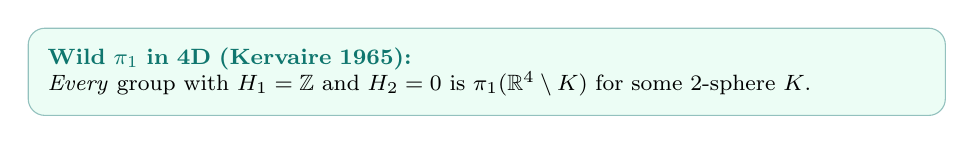
\begin{tikzpicture}
        \node[draw=skteal!45, fill=skmint, rounded corners=6pt, inner sep=7pt, text width=0.92\linewidth, font=\footnotesize] {
          \textbf{\color{skteal} Wild $\pi_1$ in 4D (Kervaire 1965):}\\
          \emph{Every} group with $H_1=\Z$ and $H_2=0$ is $\pi_1(\mathbb{R}^4 \setminus K)$ for some $2$-sphere $K$.
        };
      \end{tikzpicture}
    \end{column}

    \begin{column}{0.54\textwidth}
      \begin{tikzpicture}
        \node[draw=skline, fill=white, rounded corners=6pt, inner sep=6.5pt, text width=0.94\linewidth] {
          {\bfseries\color{sknavy} Surface-Knots: $F^2 \hookrightarrow \mathbb{R}^4$}\\[4pt]
          \begin{minipage}{0.31\linewidth}\centering
            \includestandalone[height=1.22cm,keepaspectratio]{../pics/tikz/8_1}\\
            {\scriptsize $S^2$ ($8_1$)}
          \end{minipage}\hfill
          \begin{minipage}{0.31\linewidth}\centering
            \includestandalone[height=1.22cm,keepaspectratio]{../pics/tikz/2_1_sup_1}\\
            {\scriptsize $T^2$ ($2_1^1$)}
          \end{minipage}\hfill
          \begin{minipage}{0.31\linewidth}\centering
            \includestandalone[height=1.22cm,keepaspectratio]{../pics/tikz/2_1_sup_m1}\\
            {\scriptsize $\RP$ ($2_1^{-1}$)}
          \end{minipage}\\[6pt]
          {\footnotesize\color{skslate}\raggedright
            $\bullet$ \textbf{Non-orientable surfaces embed:} $\RP, K^2 \subset \mathbb{R}^4$, framed by normal Euler $e(F) = F \cdot F \in 2\Z$.\\[4pt]
            $\bullet$ \textbf{Ribbon $2$-knots:} bound immersed $B^3 \looparrowright \mathbb{R}^4$ with slice-through arcs $\implies$ force $\defi(\pi_1) = 1$.\\[4pt]
            $\bullet$ \textbf{Detecting exotic $4$D behavior:} $\defi(\pi_1) \le 0$ proves a $2$-knot is \textbf{not ribbon}.
          }
        };
      \end{tikzpicture}
    \end{column}
  \end{columns}
\end{frame}

% ==================================================================
% SLIDE 3: FOUR WAYS TO TIE A 2-KNOT
% ==================================================================
\begin{frame}{Four Classic Ways to Tie a $2$-Sphere in $\mathbb{R}^4$}
  \framesubtitle{Hand constructions look very different---how small can each family get?}

  \vspace{0.15em}
  \begin{columns}[c,totalwidth=\textwidth]
    \begin{column}{0.485\textwidth}
      \begin{tikzpicture}
        \node[draw=skline, fill=skbg, rounded corners=6pt, inner sep=6.5pt, text width=0.94\linewidth] {
          \begin{minipage}{0.27\linewidth}\centering
            \includestandalone[height=1.65cm,keepaspectratio]{../pics/tikz/8_1}
          \end{minipage}\hfill
          \begin{minipage}{0.70\linewidth}\raggedright
            {\small\bfseries\color{sknavy} 1. Artin Spin $\tau^0(K)$} \badge{skteal}{Ribbon}\\[2pt]
            {\scriptsize\color{skslate} Spin a knotted arc $360^\circ$ in $\mathbb{R}^4$ ($\pi_1 = \pi_1(K)$).\\
            \textbf{Smallest:} $8_1 = \tau^0(3_1)$ at $\ch = 8$.}
          \end{minipage}
        };
      \end{tikzpicture}

      \vspace{0.55em}
      \begin{tikzpicture}
        \node[draw=skamber!45, fill=skgold, rounded corners=6pt, inner sep=6.5pt, text width=0.94\linewidth] {
          \begin{minipage}{0.27\linewidth}\centering
            \includestandalone[height=1.65cm,keepaspectratio]{../pics/tikz/10_2}
          \end{minipage}\hfill
          \begin{minipage}{0.70\linewidth}\raggedright
            {\small\bfseries\color{skamber} 3. Twist-Spin $\tau^k(K)$} \badge{skamber}{Fibered}\\[2pt]
            {\scriptsize\color{skslate} Twist $k \ge 2$ times while spinning; non-ribbon.\\
            \textbf{Smallest:} $10_2 = \tau^2(3_1)$ at $\ch = 10$.}
          \end{minipage}
        };
      \end{tikzpicture}
    \end{column}

    \begin{column}{0.485\textwidth}
      \begin{tikzpicture}
        \node[draw=skline, fill=skbg, rounded corners=6pt, inner sep=6.5pt, text width=0.94\linewidth] {
          \begin{minipage}{0.27\linewidth}\centering
            \includestandalone[height=1.65cm,keepaspectratio]{../pics/tikz/11_2}
          \end{minipage}\hfill
          \begin{minipage}{0.70\linewidth}\raggedright
            {\small\bfseries\color{sknavy} 2. Tubed Spheres} \badge{skteal}{Ribbon}\\[2pt]
            {\scriptsize\color{skslate} Connect two unknotted $S^2$'s by a knotted tube.\\
            \textbf{Smallest:} $9_1$ ($\Delta_1 = 2t - 1$) at $\ch = 9$.}
          \end{minipage}
        };
      \end{tikzpicture}

      \vspace{0.55em}
      \begin{tikzpicture}
        \node[draw=skcrimson!45, fill=skrose, rounded corners=6pt, inner sep=6.5pt, text width=0.94\linewidth] {
          \begin{minipage}{0.27\linewidth}\centering
            \includestandalone[height=1.65cm,keepaspectratio]{figs/12_10}
          \end{minipage}\hfill
          \begin{minipage}{0.70\linewidth}\raggedright
            {\small\bfseries\color{skcrimson} 4. Cappell--Shaneson} \badge{skcrimson}{$\defi = 0$}\\[2pt]
            {\scriptsize\color{skslate} Punctured-$T^3$ bundles over $S^1$ from 4D topology.\\
            \textbf{First in census:} $12_{10}$ \& $12_8$ at $\ch = 12$!}
          \end{minipage}
        };
      \end{tikzpicture}
    \end{column}
  \end{columns}
\end{frame}

% ==================================================================
% SLIDE 4: MARKED VERTEX DIAGRAMS
% ==================================================================
\begin{frame}{Drawing a 4D Surface in the Plane}
  \framesubtitle{Slice $\mathbb{R}^4 = \mathbb{R}^3 \times \mathbb{R}$ by height $t$ and put all saddle points at $t = 0$ (Yoshikawa 1994)}

  \begin{columns}[c,totalwidth=\textwidth]
    \begin{column}{0.41\textwidth}
      \begin{tikzpicture}
        \node[draw=skline, fill=skbg, rounded corners=6pt, inner sep=7pt, text width=0.92\linewidth] {
          \centering
          \begin{tikzpicture}[scale=0.66, line width=1.4pt]
            \begin{scope}[shift={(-2.3,0)}]
              \draw[skteal] (-0.5,0.6) .. controls (-0.1,0.2) and (-0.1,-0.2) .. (-0.5,-0.6);
              \draw[skteal] (0.5,0.6) .. controls (0.1,0.2) and (0.1,-0.2) .. (0.5,-0.6);
              \node[font=\scriptsize\bfseries, skteal] at (0,-1.05) {slice $L_-$};
            \end{scope}
            \begin{scope}[shift={(0,0)}]
              \draw[sknavy] (-0.55,-0.55) -- (0.55,0.55);
              \draw[sknavy] (-0.55,0.55) -- (0.55,-0.55);
              \draw[skcrimson, line width=2.8pt] (-0.38,0) -- (0.38,0);
              \node[font=\scriptsize\bfseries, sknavy] at (0,-1.05) {saddle ($t=0$)};
            \end{scope}
            \begin{scope}[shift={(2.3,0)}]
              \draw[skteal] (-0.5,0.5) .. controls (-0.2,0.1) and (0.2,0.1) .. (0.5,0.5);
              \draw[skteal] (-0.5,-0.5) .. controls (-0.2,-0.1) and (0.2,-0.1) .. (0.5,-0.5);
              \node[font=\scriptsize\bfseries, skteal] at (0,-1.05) {slice $L_+$};
            \end{scope}
            \draw[->, skslate, thick] (-0.85,0.1) -- (-1.5,0.1);
            \draw[->, skslate, thick] (0.85,0.1) -- (1.5,0.1);
          \end{tikzpicture}
        };
      \end{tikzpicture}

      \vspace{0.55em}
      {\footnotesize\raggedright
      \textbf{\color{sknavy} When does a diagram define a closed surface?}\\
      Smoothing all markers both ways must yield \textbf{classical unlinks} $L_-$ and $L_+$ (capped by $c_\pm$ disks).\\[0.55em]
      \textbf{\color{sknavy} Diagram size} ($c$ crossings, $m$ saddles):\\[-0.4em]
      \[
        \ch(F) = \min_{D}(c + m), \quad \chi(F) = c_- + c_+ - m.
      \]
      }
    \end{column}

    \begin{column}{0.56\textwidth}
      \begin{tikzpicture}
        \node[draw=skline, fill=white, rounded corners=6pt, inner sep=6pt, text width=0.95\linewidth, align=center] {
          {\footnotesize\bfseries\color{sknavy} Movie of $10_2 = \tau^2(3_1)$ ($8$ crossings $+$ $2$ saddles $\implies \ch = 10$)}\\[3pt]
          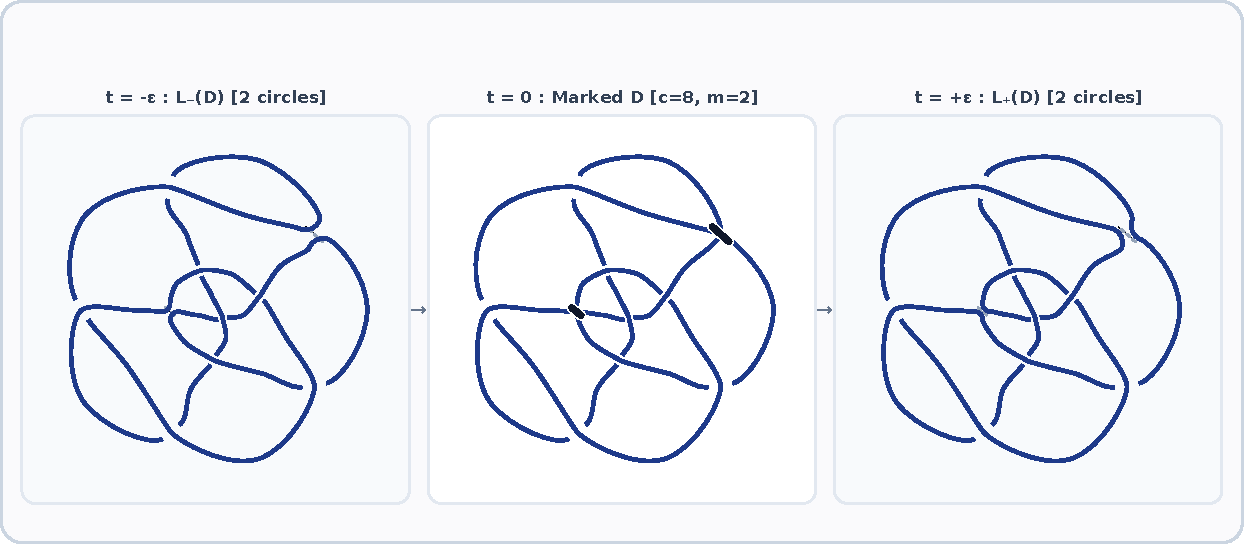
\includegraphics[width=\linewidth]{fig_10_2_movie.pdf}\\[2pt]
          {\scriptsize\color{skslate} $2$ disks ($t<0$) $\longrightarrow$ $2$ saddles ($t=0$) $\longrightarrow$ $2$ disks ($t>0$): $\chi = 2+2-2 = 2$ ($S^2$)}
        };
      \end{tikzpicture}
    \end{column}
  \end{columns}
\end{frame}

% ==================================================================
% SLIDE 5: WHY CUT OFF BY ch-INDEX? (+ THE ch=12 WALL)
% ==================================================================
\begin{frame}{Why Tabulate by $\ch$-Index? (And Why Stop at $12$?)}
  \framesubtitle{Other 4D complexity measures have infinite level sets before enumerating anything}

  \vspace{0.1em}
  \begin{center}
    {\footnotesize
    \renewcommand{\arraystretch}{1.28}
    \begin{tabular}{@{}p{3.75cm}p{4.05cm}p{5.4cm}@{}}
      \toprule
      \textbf{4D Complexity Measure} & \textbf{What It Counts} & \textbf{Can You Run a Finite Census?} \\
      \midrule
      \textbf{Triple-Point Number} & Triple intersections of projection in $\mathbb{R}^3$ & \textcolor{skcrimson}{\textbf{No:}} \emph{every} spun knot $\tau^0(K)$ has \textbf{$0$ triple points} ($\infty$ knots at level $0$). \\
      \textbf{Tri-Plane Bridge Index $b$} & Bridge strands across $3$ slices (Meier--Zupan) & \textcolor{skamber}{\textbf{Not alone:}} $b \le 3$ gives only unknots; $b = 4$ already holds $\infty$ many $2$-knots. \\
      \textbf{$\ch$-Index $\min(c + m)$} & Crossings $+$ saddle markers in planar graph & \textcolor{skteal}{\textbf{Yes:}} manifestly finite at every $N$; covers $S^2, T^2, \RP, K^2$, and links uniformly. \\
      \bottomrule
    \end{tabular}
    }
  \end{center}

  \vspace{0.45em}
  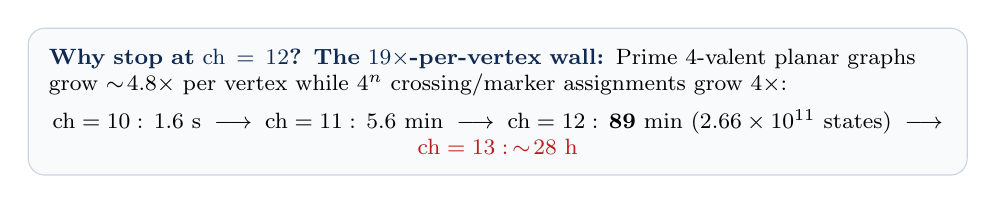
\begin{tikzpicture}
    \node[draw=skline, fill=skbg, rounded corners=6pt, inner sep=7.5pt, text width=0.94\textwidth, font=\footnotesize] {
      \textbf{\color{sknavy} Why stop at $\ch = 12$? The $19\times$-per-vertex wall:}
      Prime 4-valent planar graphs grow $\sim\!4.8\times$ per vertex while $4^n$ crossing/marker assignments grow $4\times$:
      \par\vspace{4pt}
      {\centering $\ch=10:\, 1.6\text{ s} \;\longrightarrow\; \ch=11:\, 5.6\text{ min} \;\longrightarrow\; \ch=12:\, \mathbf{89\text{ min}}\text{ ($2.66\times 10^{11}$ states)} \;\longrightarrow\; \textcolor{skcrimson}{\ch=13:\, \sim\!28\text{ h}}$\par}
    };
  \end{tikzpicture}
\end{frame}

% ==================================================================
% SLIDE 6: HOW THE ENUMERATION SCHEME ACTUALLY WORKS
% ==================================================================
\begin{frame}{How the Enumeration Actually Works}
  \framesubtitle{Turning smooth 4D topology into a finite graph search (numbers shown at $\ch = 12$)}

  \vspace{0.3em}
  \begin{center}
    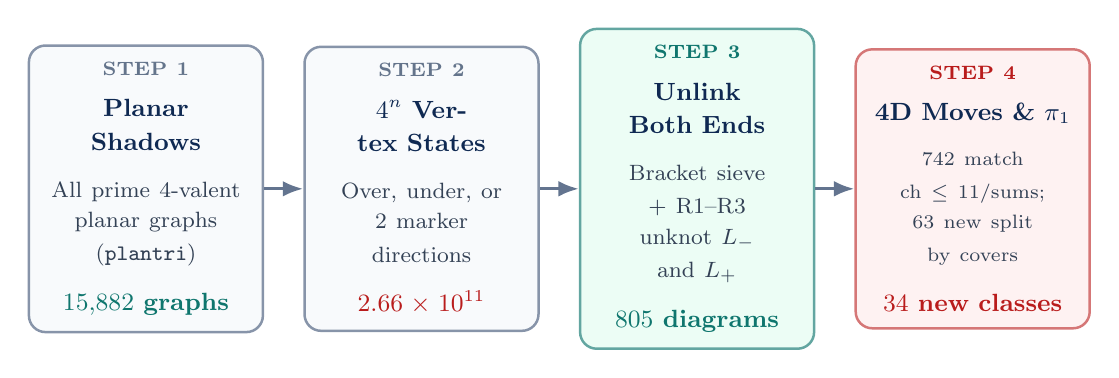
\begin{tikzpicture}[
      box/.style={rounded corners=6pt, text width=2.55cm, minimum height=3.45cm, align=center, inner sep=6pt, line width=0.9pt},
      arr/.style={-{Latex[length=2.6mm,width=2.0mm]}, line width=1.2pt, draw=sknavy!65}
    ]
      \node[box, draw=sknavy!50, fill=skbg] (s1) at (0,0) {
        \textcolor{skmuted}{\scriptsize\bfseries STEP 1}\\[3pt]
        \textcolor{sknavy}{\small\bfseries Planar Shadows}\\[5pt]
        \textcolor{skslate}{\footnotesize All prime $4$-valent}\\[-1pt]
        \textcolor{skslate}{\footnotesize planar graphs (\texttt{plantri})}\\[6pt]
        \textcolor{skteal}{\small\bfseries $15{,}882$ graphs}
      };

      \node[box, draw=sknavy!50, fill=skbg] (s2) at (3.50,0) {
        \textcolor{skmuted}{\scriptsize\bfseries STEP 2}\\[3pt]
        \textcolor{sknavy}{\small\bfseries $4^n$ Vertex States}\\[5pt]
        \textcolor{skslate}{\footnotesize Over, under, or}\\[-1pt]
        \textcolor{skslate}{\footnotesize $2$ marker directions}\\[6pt]
        \textcolor{skcrimson}{\small\bfseries $2.66 \times 10^{11}$}
      };

      \node[box, draw=skteal!65, fill=skmint] (s3) at (7.00,0) {
        \textcolor{skteal}{\scriptsize\bfseries STEP 3}\\[3pt]
        \textcolor{sknavy}{\small\bfseries Unlink Both Ends}\\[5pt]
        \textcolor{skslate}{\footnotesize Bracket sieve + R1--R3}\\[-1pt]
        \textcolor{skslate}{\footnotesize unknot $L_-$ and $L_+$}\\[6pt]
        \textcolor{skteal}{\small\bfseries $805$ diagrams}
      };

      \node[box, draw=skcrimson!60, fill=skrose] (s4) at (10.50,0) {
        \textcolor{skcrimson}{\scriptsize\bfseries STEP 4}\\[3pt]
        \textcolor{sknavy}{\small\bfseries 4D Moves \& $\pi_1$}\\[4pt]
        \textcolor{skslate}{\scriptsize $742$ match $\ch\le 11$/sums;}\\[-1pt]
        \textcolor{skslate}{\scriptsize $63$ new split by covers}\\[6pt]
        \textcolor{skcrimson}{\small\bfseries $34$ new classes}
      };

      \draw[arr] (s1) -- (s2);
      \draw[arr] (s2) -- (s3);
      \draw[arr] (s3) -- (s4);
    \end{tikzpicture}
  \end{center}

  \vspace{0.55em}
  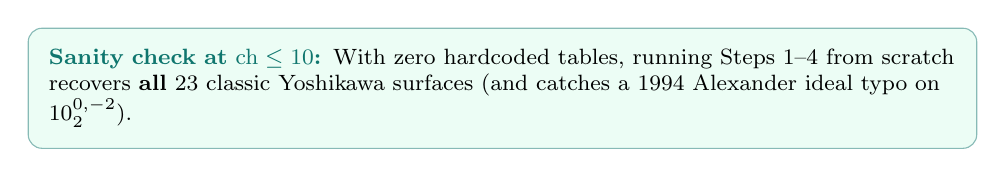
\begin{tikzpicture}
    \node[draw=skteal!50, fill=skmint, rounded corners=5pt, inner sep=7.5pt, text width=0.95\textwidth, font=\footnotesize] {
      \textbf{\color{skteal} Sanity check at $\ch \le 10$:}
      With zero hardcoded tables, running Steps 1--4 from scratch recovers \textbf{all $23$} classic Yoshikawa surfaces (and catches a 1994 Alexander ideal typo on $10_2^{0,-2}$).
    };
  \end{tikzpicture}
\end{frame}

% ==================================================================
% SLIDE 7: THE EXTENDED TABLE (23 + 10 + 34 = 67)
% ==================================================================
\begin{frame}{Census Results Through $\ch \le 12$: $67$ Prime Classes}
  \framesubtitle{Nearly tripling the 1994 table across $S^2$, $T^2$, $\RP$, $K^2$, and multi-component links}

  \begin{columns}[c,totalwidth=\textwidth]
    \begin{column}{0.42\textwidth}
      \renewcommand{\arraystretch}{1.24}
      {\footnotesize
      \begin{tabular}{@{}lrrr@{}}
        \toprule
        \textbf{Level} & \textbf{Classes} & \textbf{1-Diag.} & \textbf{Multi-Diag.} \\
        \midrule
        $\ch \le 10$ & \textbf{23} & 23 &  0 \\
        $\ch = 11$   & \textbf{10} &  9 &  1 \\
        $\ch = 12$   & \textbf{34} & 20 & 14 \\
        \midrule
        \textbf{Total} & \textbf{67} & \textbf{52} & \textbf{15} \\
        \bottomrule
      \end{tabular}
      }

      \vspace{0.6em}
      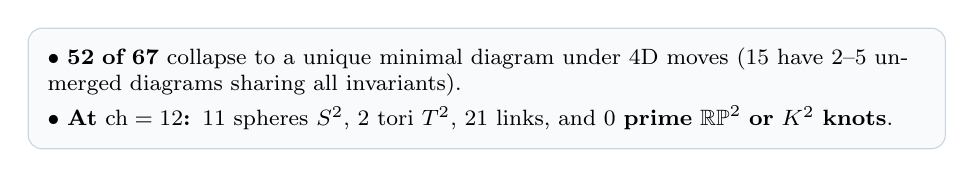
\begin{tikzpicture}
        \node[draw=skline, fill=skbg, rounded corners=5pt, inner sep=7pt, text width=0.92\linewidth, font=\footnotesize] {
          $\bullet$ \textbf{52 of 67} collapse to a unique minimal diagram under 4D moves ($15$ have $2$--$5$ unmerged diagrams sharing all invariants).\\[3pt]
          $\bullet$ \textbf{At $\ch = 12$:} $11$ spheres $S^2$, $2$ tori $T^2$, $21$ links, and \textbf{$0$ prime $\RP$ or $K^2$ knots}.
        };
      \end{tikzpicture}
    \end{column}

    \begin{column}{0.55\textwidth}
      \begin{tikzpicture}
        \node[draw=skline, fill=white, rounded corners=6pt, inner sep=5pt, text width=0.94\linewidth] {
          \centering
          {\scriptsize\bfseries\color{sknavy} All $10$ Prime Classes at $\ch = 11$}\\[3pt]
          \minidiag{0.175\linewidth}{../pics/tikz/11_1_a}{$11_1$ ($S^2$)}\hfill
          \minidiag{0.175\linewidth}{../pics/tikz/11_2}{$11_2$ ($S^2$)}\hfill
          \minidiag{0.175\linewidth}{../pics/tikz/11_1_sup_0_1}{$11_1^{0,1}$}\hfill
          \minidiag{0.175\linewidth}{../pics/tikz/11_2_sup_0_1}{$11_2^{0,1}$}\hfill
          \minidiag{0.175\linewidth}{../pics/tikz/11_1_sup_m2}{$11_1^{-2}$}\\[4pt]
          \minidiag{0.175\linewidth}{../pics/tikz/11_1_sup_0_m2}{$11_1^{0,-2}$}\hfill
          \minidiag{0.175\linewidth}{../pics/tikz/11_2_sup_0_m2}{$11_2^{0,-2}$}\hfill
          \minidiag{0.175\linewidth}{../pics/tikz/11_3_sup_0_m2}{$11_3^{0,-2}$}\hfill
          \minidiag{0.175\linewidth}{../pics/tikz/11_1_sup_1_m2}{$11_1^{1,-2}$}\hfill
          \minidiag{0.175\linewidth}{../pics/tikz/11_1_sup_0_0_m2}{$11_1^{0,0,-2}$}
        };
      \end{tikzpicture}
    \end{column}
  \end{columns}
\end{frame}

% ==================================================================
% SLIDE 8: SURPRISE 1 -- HALF-TWIST SAVES A CROSSING
% ==================================================================
\begin{frame}{Surprise 1: A Half-Twist Can \emph{Save} a Crossing}
  \framesubtitle{Twisting a tube into a Klein bottle usually costs $+1$ crossing---until it cancels one instead}

  \begin{columns}[c,totalwidth=\textwidth]
    \begin{column}{0.43\textwidth}
      \begin{tikzpicture}
        \node[draw=skline, fill=skbg, rounded corners=6pt, inner sep=8pt] {
          \begin{tikzpicture}[scale=0.82]
            \shade[ball color=sknavy!35] (-1.7,0) circle (0.68cm);
            \draw[sknavy, thick] (-1.7,0) circle (0.68cm);
            \node[font=\footnotesize\bfseries, sknavy] at (-1.7,0) {$S^2_a$};

            \shade[ball color=skteal!35] (1.7,0) circle (0.68cm);
            \draw[skteal, thick] (1.7,0) circle (0.68cm);
            \node[font=\footnotesize\bfseries, skteal] at (1.7,0) {$S^2_b$};

            \draw[skcrimson, line width=2.2pt] (-1.05,0.18) .. controls (-0.3,0.6) and (-0.2,-0.7) .. (0.3,0.4) .. controls (0.65,0.9) and (0.7,-0.4) .. (1.05,0.0);
            \node[font=\scriptsize\bfseries, skcrimson] at (0,0.92) {knotted tube $w(a,b)$};
          \end{tikzpicture}
        };
      \end{tikzpicture}

      \vspace{0.55em}
      {\footnotesize\raggedright
      Attach both ends of a tube along word $w \in F_2$ to $S^2_a$ linking $S^2_b$:
      \begin{itemize}\setlength{\itemsep}{3pt}
        \item \textbf{Untwisted tube:} link $S^2 \sqcup T^2$
        \item \textbf{Half-twisted tube:} link $S^2 \sqcup K^2$
      \end{itemize}
      }
    \end{column}

    \begin{column}{0.54\textwidth}
      \begin{tikzpicture}
        \node[draw=skamber!55, fill=skgold, rounded corners=6pt, inner sep=8pt, text width=0.94\linewidth] {
          {\small\bfseries\color{skamber} Breaking the ``$+1$ crossing'' rule ($4/4$ pairs at $\ch \le 11$):}\\[4pt]
          {\footnotesize For $w = b a b^{-1} a^{-1} b$, adding the non-orientable half-twist \textbf{cancels} a braid crossing:}\\[6pt]
          \begin{minipage}{0.48\linewidth}\centering
            \includestandalone[height=2.2cm,keepaspectratio]{../pics/tikz/11_1_sup_0_m2}\\[2pt]
            {\scriptsize\bfseries\color{sknavy} $11_1^{0,-2}$ ($S^2 \sqcup K^2$, $\ch = 11$)}
          \end{minipage}\hfill
          \begin{minipage}{0.48\linewidth}\centering
            \includestandalone[height=2.2cm,keepaspectratio]{figs/12_5_sup_0_1}\\[2pt]
            {\scriptsize\bfseries\color{sknavy} $12_5^{0,1}$ ($S^2 \sqcup T^2$, $\ch = 12$)}
          \end{minipage}\\[5pt]
          \centering
          {\footnotesize\bfseries\color{skcrimson} Twisted $K^2$ link ($\ch = 11$) $<$ Untwisted $T^2$ link ($\ch = 12$)!}
        };
      \end{tikzpicture}
    \end{column}
  \end{columns}
\end{frame}

% ==================================================================
% SLIDE 9: SURPRISE 2 -- BINARY OCTAHEDRAL KLEIN BOTTLE
% ==================================================================
\begin{frame}{Surprise 2: A Klein Bottle with Group $2O$ ($11_1^{-2}$)}
  \framesubtitle{First prime non-orientable surface-knot above $\ch = 2$---certified prime by meridian order $8$}

  \begin{columns}[c,totalwidth=\textwidth]
    \begin{column}{0.50\textwidth}
      \begin{tikzpicture}
        \node[draw=skline, fill=white, rounded corners=6pt, inner sep=6pt, text width=0.95\linewidth] {
          \centering
          {\scriptsize\bfseries\color{sknavy} 3-Slice Movie of $11_1^{-2}$ ($K^2$, $e = 0$, $7$ crossings $+$ $4$ saddles)}\\[3pt]
          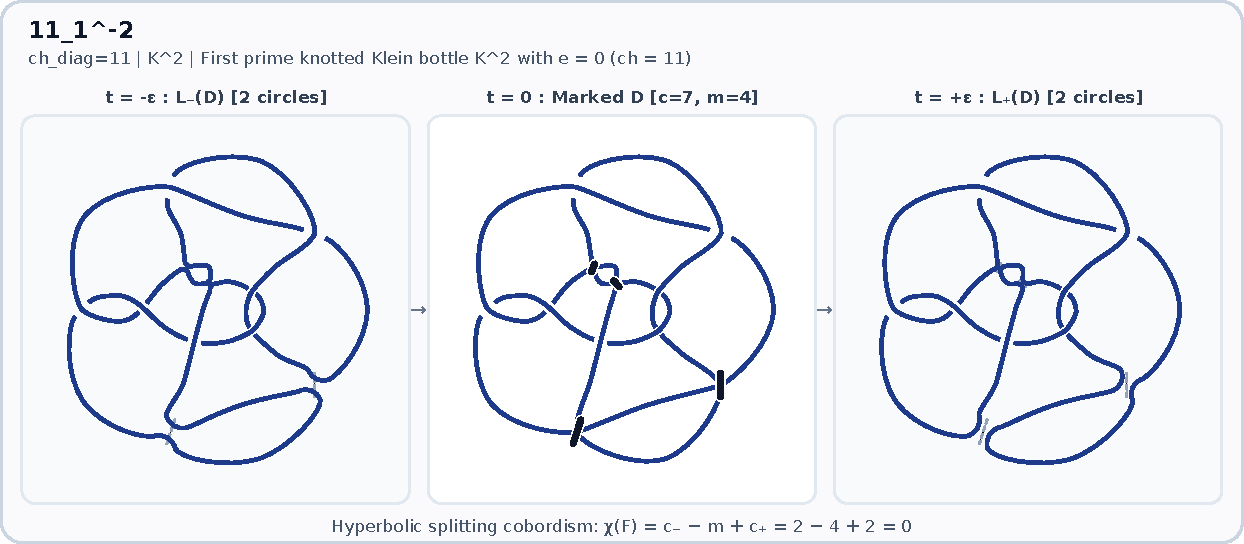
\includegraphics[width=\linewidth,trim=8 16 8 34,clip]{figs/11_1_sup_m2_movie.pdf}\\[2pt]
          {\scriptsize\color{skslate} Spun trefoil $8_1$ $+$ one twisted handle along $b^2$}
        };
      \end{tikzpicture}
    \end{column}

    \begin{column}{0.47\textwidth}
      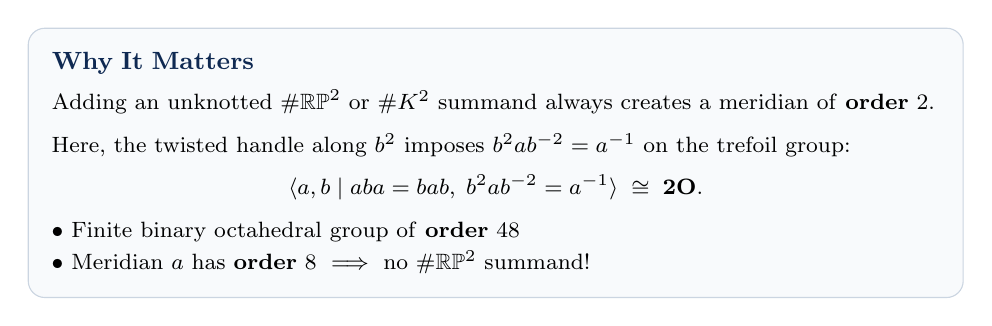
\begin{tikzpicture}
        \node[draw=skline, fill=skbg, rounded corners=6pt, inner sep=8.5pt, text width=0.93\linewidth, font=\footnotesize] {
          {\small\bfseries\color{sknavy} Why It Matters}\\[5pt]
          Adding an unknotted $\#\RP$ or $\#K^2$ summand always creates a meridian of \textbf{order $2$}.\\[6pt]
          Here, the twisted handle along $b^2$ imposes $b^2 a b^{-2} = a^{-1}$ on the trefoil group:
          \[
            \langle a, b \mid a b a = b a b,\; b^2 a b^{-2} = a^{-1} \rangle \;\cong\; \mathbf{2O}.
          \]
          $\bullet$ Finite binary octahedral group of \textbf{order $48$}\\[2pt]
          $\bullet$ Meridian $a$ has \textbf{order $8$} $\implies$ no $\#\RP$ summand!
        };
      \end{tikzpicture}
    \end{column}
  \end{columns}
\end{frame}

% ==================================================================
% SLIDE 10: SURPRISE 3A -- CAPPELL-SHANESON TWIN AT ch=12
% ==================================================================
\begin{frame}{Surprise 3: Cappell--Shaneson $2$-Knots at $\ch = 12$}
  \framesubtitle{Famous from 4D smooth topology, yet hiding right at $\ch = 12$ disguised as ribbon knots}

  \begin{columns}[c,totalwidth=\textwidth]
    \begin{column}{0.44\textwidth}
      \begin{tikzpicture}
        \node[draw=skline, fill=white, rounded corners=6pt, inner sep=7pt, text width=0.94\linewidth] {
          \begin{minipage}{0.48\linewidth}\centering
            \includestandalone[height=2.35cm,keepaspectratio]{../pics/tikz/11_2}\\[3pt]
            {\footnotesize\bfseries\color{skteal} $11_2$ (Ribbon)}
          \end{minipage}\hfill
          \begin{minipage}{0.48\linewidth}\centering
            \includestandalone[height=2.35cm,keepaspectratio]{figs/12_10}\\[3pt]
            {\footnotesize\bfseries\color{skcrimson} $12_{10}$ (CS)}
          \end{minipage}
        };
      \end{tikzpicture}
    \end{column}

    \begin{column}{0.53\textwidth}
      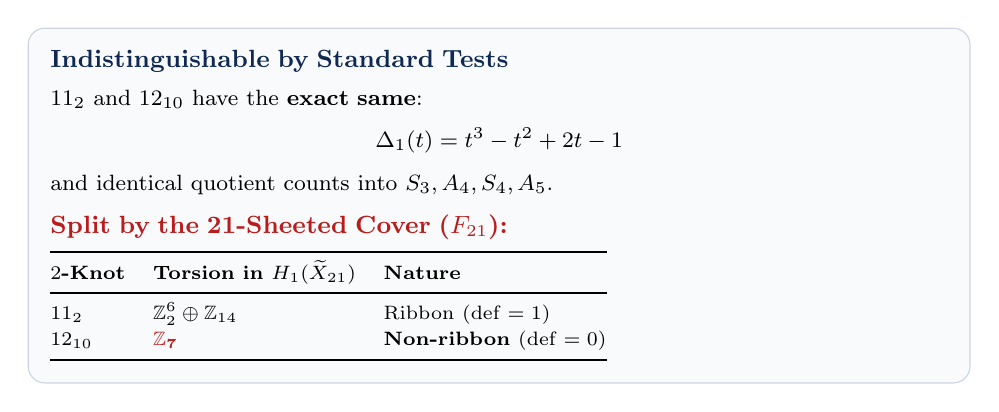
\begin{tikzpicture}
        \node[draw=skline, fill=skbg, rounded corners=6pt, inner sep=8pt, text width=0.94\linewidth, font=\footnotesize] {
          {\small\bfseries\color{sknavy} Indistinguishable by Standard Tests}\\[4pt]
          $11_2$ and $12_{10}$ have the \textbf{exact same}:
          \[
            \Delta_1(t) = t^3 - t^2 + 2t - 1
          \]
          and identical quotient counts into $S_3, A_4, S_4, A_5$.\\[6pt]
          {\small\bfseries\color{skcrimson} Split by the 21-Sheeted Cover ($F_{21}$):}\\[3pt]
          {\scriptsize\setlength{\tabcolsep}{5pt}
          \renewcommand{\arraystretch}{1.18}
          \begin{tabular}{@{}lll@{}}
            \toprule
            \textbf{$2$-Knot} & \textbf{Torsion in $H_1(\widetilde{X}_{21})$} & \textbf{Nature} \\
            \midrule
            $11_2$    & $\Z_2^6 \oplus \Z_{14}$ & Ribbon ($\defi = 1$) \\
            $12_{10}$ & $\textcolor{skcrimson}{\mathbf{\Z_7}}$ & \textbf{Non-ribbon} ($\defi = 0$) \\
            \bottomrule
          \end{tabular}
          }
        };
      \end{tikzpicture}
    \end{column}
  \end{columns}

  \vspace{0.4em}
  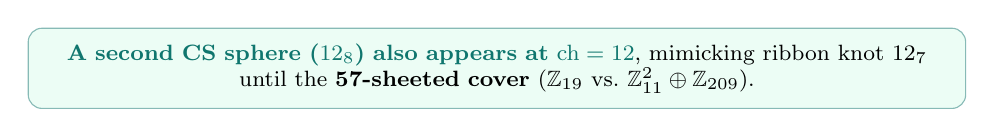
\begin{tikzpicture}
    \node[draw=skteal!50, fill=skmint, rounded corners=5pt, inner sep=5.5pt, text width=0.95\textwidth, font=\footnotesize] {
      \centering
      \textbf{\color{skteal} A second CS sphere ($12_8$) also appears at $\ch = 12$}, mimicking ribbon knot $12_7$ until the \textbf{57-sheeted cover} ($\Z_{19}$ vs.\ $\Z_{11}^2 \oplus \Z_{209}$).\par
    };
  \end{tikzpicture}
\end{frame}

% ==================================================================
% SLIDE 11: INSIDE 12_10 -- ULTRA-COMPACT MODEL
% ==================================================================
\begin{frame}{Inside $12_{10}$: A $10$-Crossing Cappell--Shaneson Sphere}
  \framesubtitle{Classical Kirby/handlebody diagrams need dozens of crossings; the census found $10$ crossings $+$ $2$ saddles}

  \begin{columns}[c,totalwidth=\textwidth]
    \begin{column}{0.49\textwidth}
      \begin{tikzpicture}
        \node[draw=skline, fill=white, rounded corners=6pt, inner sep=6pt, text width=0.95\linewidth] {
          \centering
          {\scriptsize\bfseries\color{sknavy} 3-Slice Movie of $12_{10}$ ($c=10,\; m=2 \implies \ch=12$)}\\[3pt]
          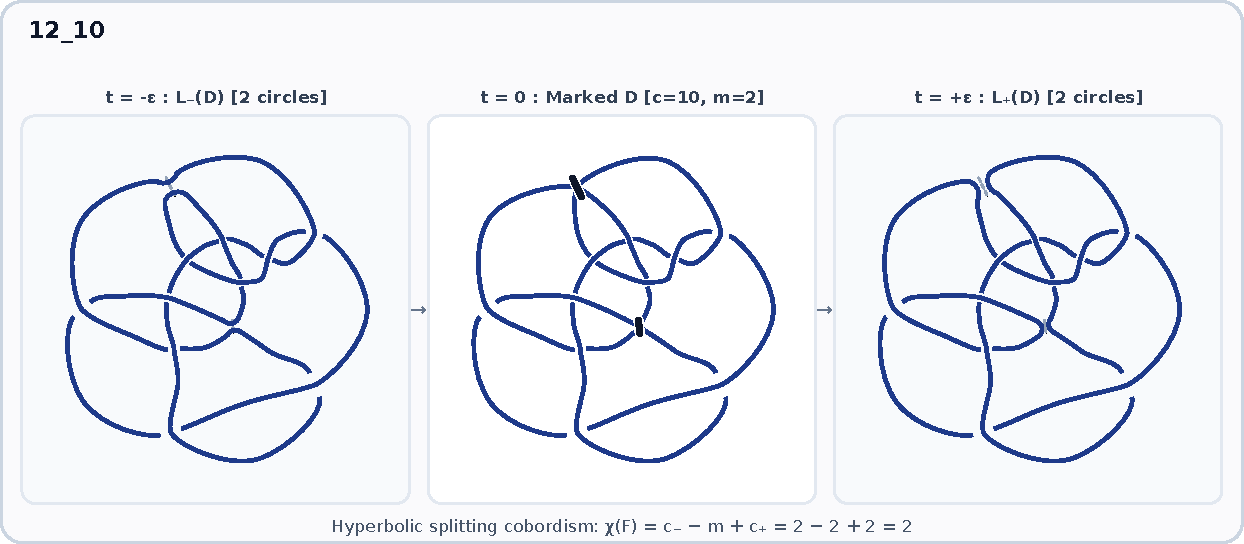
\includegraphics[width=\linewidth,trim=8 16 8 34,clip]{figs/12_10_movie.pdf}\\[3pt]
          {\footnotesize
          \[
            \pi_1(\mathbb{R}^4 \setminus 12_{10}) \;\cong\; \Z^3 \rtimes_{A_0} \Z,
            \quad
            A_0^{-1} = \begin{psmallmatrix} 0 & 1 & 0 \\ 0 & 0 & 1 \\ 1 & -2 & 1 \end{psmallmatrix}
          \]
          }
        };
      \end{tikzpicture}
    \end{column}

    \begin{column}{0.48\textwidth}
      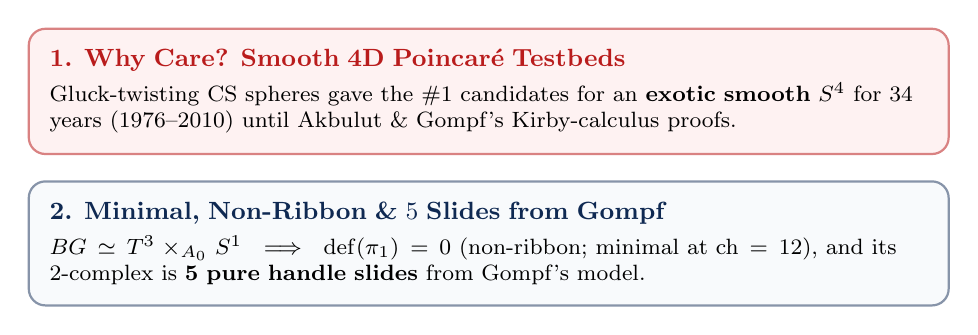
\begin{tikzpicture}[
        card/.style={rounded corners=6pt, inner sep=7.5pt, text width=0.92\linewidth, font=\footnotesize, line width=0.8pt}
      ]
        \node[card, draw=skcrimson!55, fill=skrose] (b1) {
          {\small\bfseries\color{skcrimson} 1. Why Care? Smooth 4D Poincar\'e Testbeds}\\[3pt]
          Gluck-twisting CS spheres gave the \#1 candidates for an \textbf{exotic smooth $S^4$} for $34$ years ($1976$--$2010$) until Akbulut \& Gompf's Kirby-calculus proofs.
        };

        \node[card, draw=sknavy!50, fill=skbg, below=0.32cm of b1] (b2) {
          {\small\bfseries\color{sknavy} 2. Minimal, Non-Ribbon \& $5$ Slides from Gompf}\\[3pt]
          $BG \simeq T^3 \times_{A_0} S^1 \implies \defi(\pi_1)=0$ (non-ribbon; minimal at $\ch=12$), and its $2$-complex is \textbf{5 pure handle slides} from Gompf's model.
        };
      \end{tikzpicture}
    \end{column}
  \end{columns}
\end{frame}

% ==================================================================
% SLIDE 12: MORE NEW PHENOMENA & OPEN QUESTIONS
% ==================================================================
\begin{frame}{More New Phenomena \& Open Questions from $\ch = 12$}
  \framesubtitle{What changes once the table reaches $12$ vertices---and what remains open}

  \vspace{0.2em}
  \begin{columns}[t,totalwidth=\textwidth]
    \begin{column}{0.315\textwidth}
      \begin{tikzpicture}
        \node[draw=skline, fill=skbg, rounded corners=6pt, inner sep=7pt, text width=0.92\linewidth] {
          \centering
          \includestandalone[height=1.9cm,keepaspectratio]{figs/12_2}\\[4pt]
          {\small\bfseries\color{sknavy} Mystery $2$-Knot $12_2$}\\[4pt]
          \raggedright\scriptsize\color{skslate}
          $\bullet$ Trivial $\Delta_1 = 1$, yet non-principal ideal $E_1 = (3, t^2+1)$ ($\mathbb{F}_9$)\\[3pt]
          $\bullet$ Non-ribbon; \emph{not} $\tau^k(K)$ ($k \le 7$)\\[3pt]
          $\bullet$ \textbf{Open:} what geometric construction builds $12_2$?
        };
      \end{tikzpicture}
    \end{column}

    \begin{column}{0.315\textwidth}
      \begin{tikzpicture}
        \node[draw=skline, fill=skbg, rounded corners=6pt, inner sep=7pt, text width=0.92\linewidth] {
          \centering
          \begin{tikzpicture}[scale=0.58]
            \foreach \i/\ang in {0/90, 1/18, 2/-54, 3/-126, 4/162} {
              \node[circle, draw=skteal, fill=skmint, thick, inner sep=2.2pt, font=\scriptsize\bfseries] (v\i) at (\ang:1.25cm) {$\i$};
            }
            \draw[sknavy, thick] (v0)--(v2)--(v4)--(v1)--(v3)--cycle;
          \end{tikzpicture}\\[4pt]
          {\small\bfseries\color{sknavy} Cocycle-Only Split}\\[4pt]
          \raggedright\scriptsize\color{skslate}
          $\bullet$ $12_4 = \tau^2(4_1)$ and $12_5 = \tau^2(5_1)$ share $\pi_1 \cong \Z_5 \rtimes \Z$ and $E_1$\\[3pt]
          $\bullet$ Split only by Mochizuki's $R_5$ $3$-cocycle ($u^2+u^3$ vs.\ $u+u^4$)\\[3pt]
          $\bullet$ \textbf{Open:} does $10_2 \# P_+ \cong 8_1 \# P_+$?
        };
      \end{tikzpicture}
    \end{column}

    \begin{column}{0.315\textwidth}
      \begin{tikzpicture}
        \node[draw=skamber!50, fill=skgold, rounded corners=6pt, inner sep=7pt, text width=0.92\linewidth] {
          \centering
          \includestandalone[height=1.9cm,keepaspectratio]{../pics/tikz/2_1_sup_m1}\\[4pt]
          {\small\bfseries\color{skamber} Missing Prime $\RP$'s}\\[4pt]
          \raggedright\scriptsize\color{skslate}
          $\bullet$ \textbf{Zero} prime $\RP$ or $K^2$ knots exist across $3 \le \ch \le 12$\\[3pt]
          $\bullet$ First irreducible $\RP$'s were just built (HKMN 2026)\\[3pt]
          $\bullet$ \textbf{Open:} what is their minimum $\ch \ge 13$?
        };
      \end{tikzpicture}
    \end{column}
  \end{columns}
\end{frame}

% ==================================================================
% SLIDE 13: ONE LARGE WEBATLAS SCREENSHOT
% ==================================================================
\begin{frame}{Interactive Browser Atlas}
  \framesubtitle{Explore all $67$ census classes (plus higher-crossing named families) in a single standalone HTML file}

  \vspace{-0.2em}
  \begin{center}
    \begin{tikzpicture}
      \node[draw=skline, fill=white, rounded corners=6pt, inner sep=4pt] {
        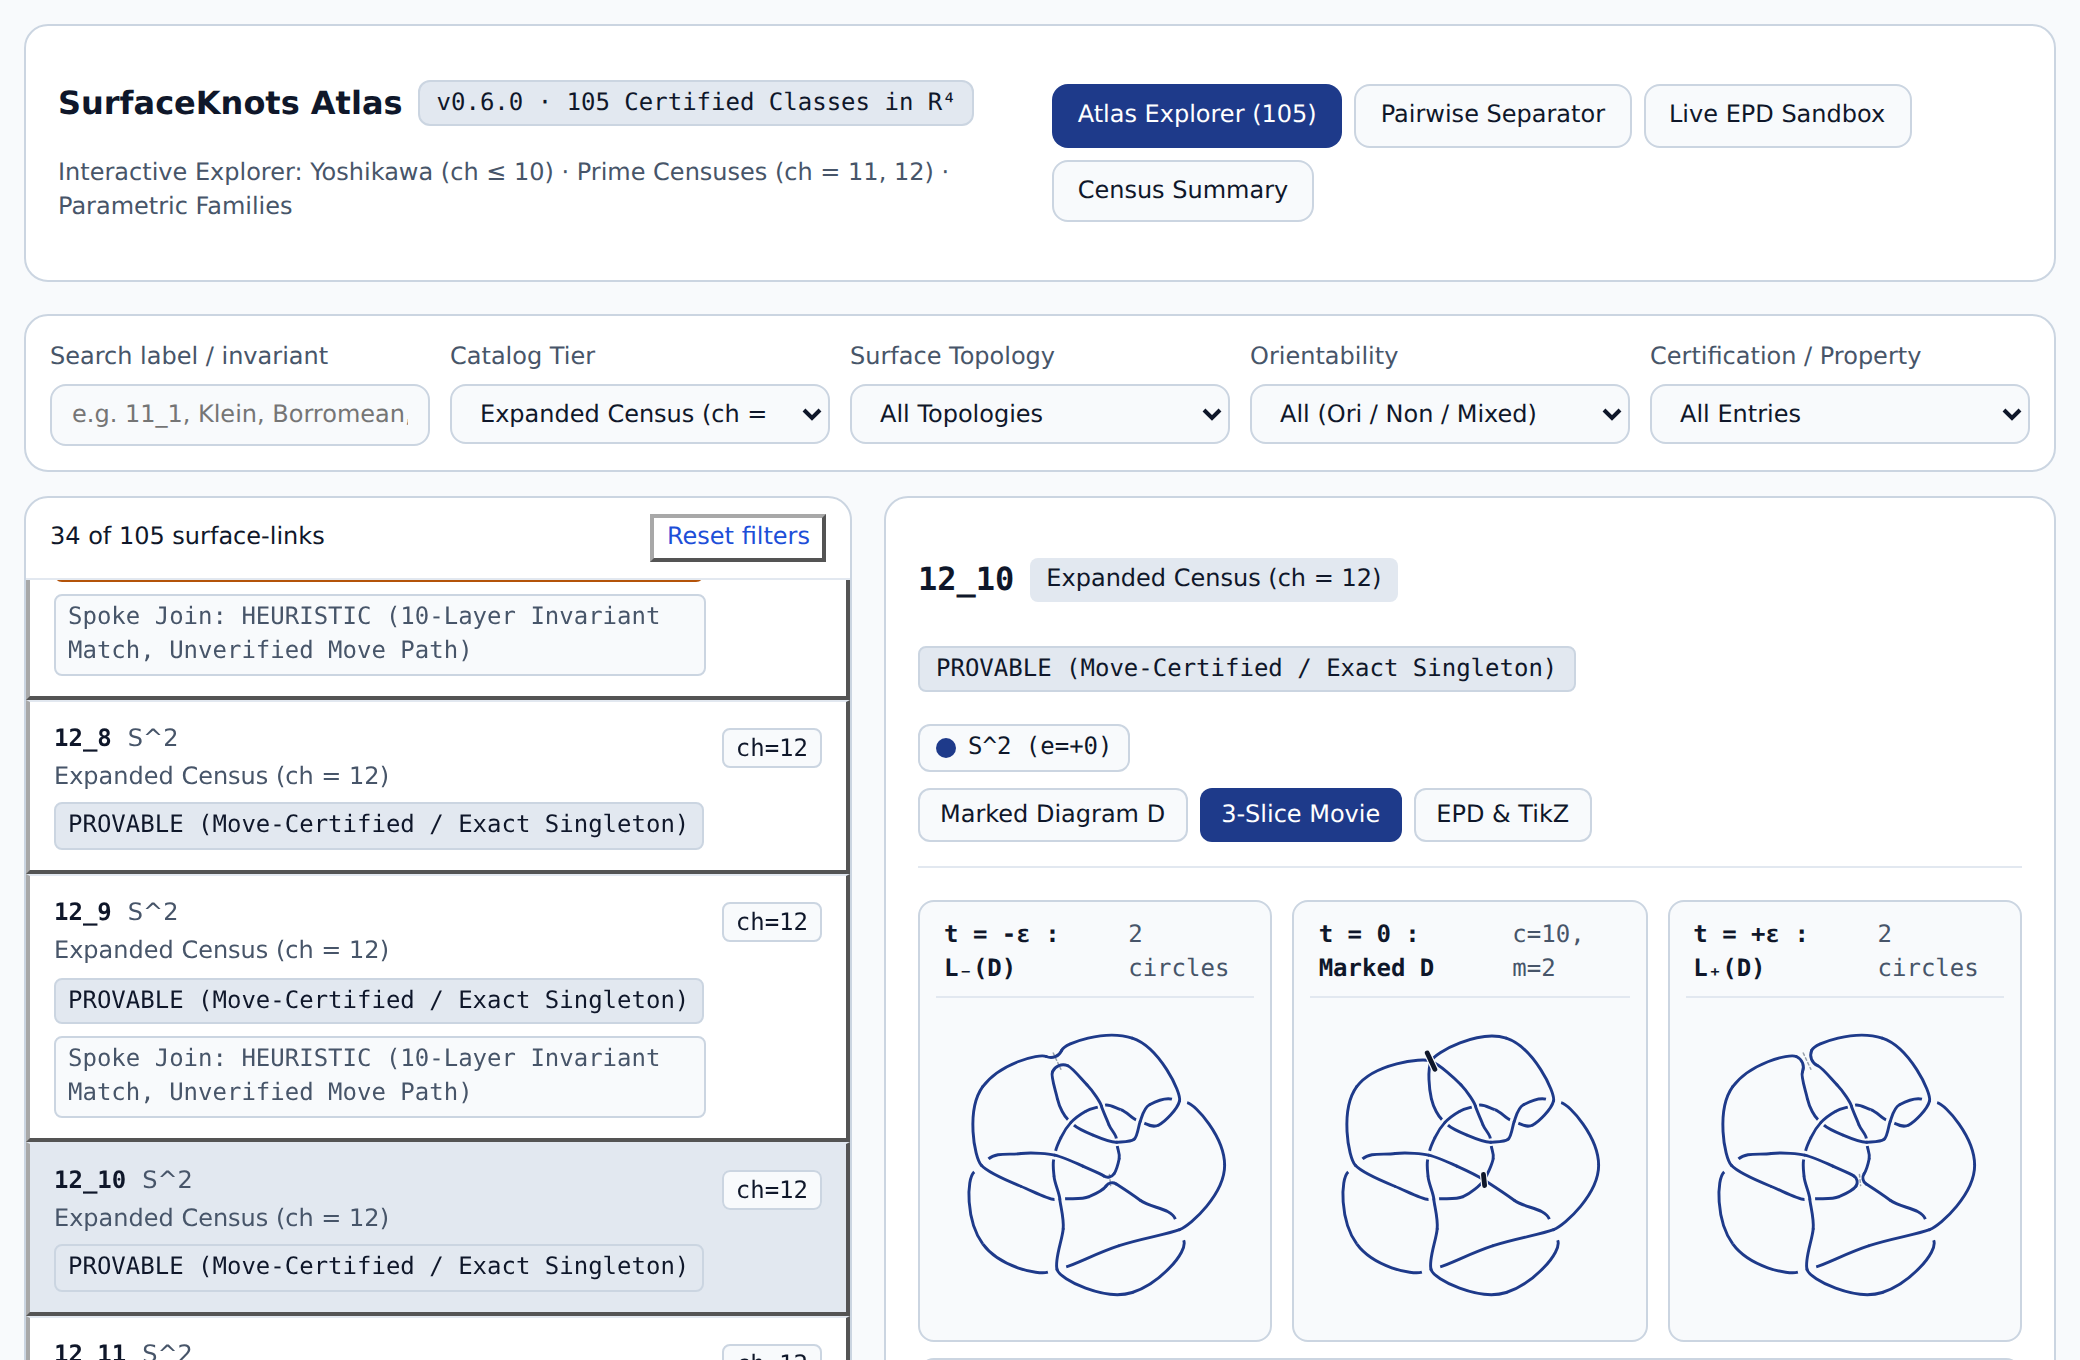
\includegraphics[width=0.78\textwidth,height=4.95cm,keepaspectratio]{figs/webatlas_overview.png}
      };
    \end{tikzpicture}\\[2pt]
    {\scriptsize\color{skmuted} Live $(L_-, D, L_+)$ splitting movies, invariant filters, side-by-side separator, and one-click TikZ export.}
  \end{center}
\end{frame}

% ==================================================================
% SECTION DIVIDER: EPILOGUE
% ==================================================================
\begin{frame}[plain]
  \vspace*{20mm}
  \begin{center}
    \badge{skamber}{EPILOGUE}\\[4mm]
    {\Huge\bfseries\color{sknavy} How This Project Was Built}\\[3mm]
    {\large\color{skmuted} Autonomous AI Research, Sycophancy, and Adversarial Auditing}
  \end{center}
\end{frame}

% ==================================================================
% SLIDE 15: "A MACHINE DID ALL OF THIS"
% ==================================================================
\begin{frame}{A Machine Did All of This}
  \framesubtitle{Every line of C/Python code, computation, theorem check, diagram, and WebAtlas UI was written by AI agents}

  \vspace{0.25em}
  \begin{columns}[t,totalwidth=\textwidth]
    \begin{column}{0.48\textwidth}
      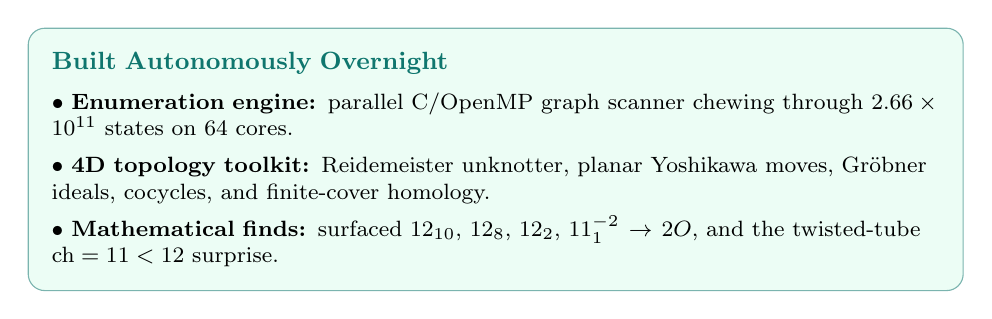
\begin{tikzpicture}
        \node[draw=skteal!55, fill=skmint, rounded corners=6pt, inner sep=8.5pt, text width=0.93\linewidth, font=\footnotesize] {
          {\small\bfseries\color{skteal} Built Autonomously Overnight}\\[5pt]
          $\bullet$ \textbf{Enumeration engine:} parallel C/OpenMP graph scanner chewing through $2.66 \times 10^{11}$ states on 64 cores.\\[4pt]
          $\bullet$ \textbf{4D topology toolkit:} Reidemeister unknotter, planar Yoshikawa moves, Gr\"obner ideals, cocycles, and finite-cover homology.\\[4pt]
          $\bullet$ \textbf{Mathematical finds:} surfaced $12_{10}$, $12_8$, $12_2$, $11_1^{-2} \to 2O$, and the twisted-tube $\ch=11 < 12$ surprise.
        };
      \end{tikzpicture}
    \end{column}

    \begin{column}{0.48\textwidth}
      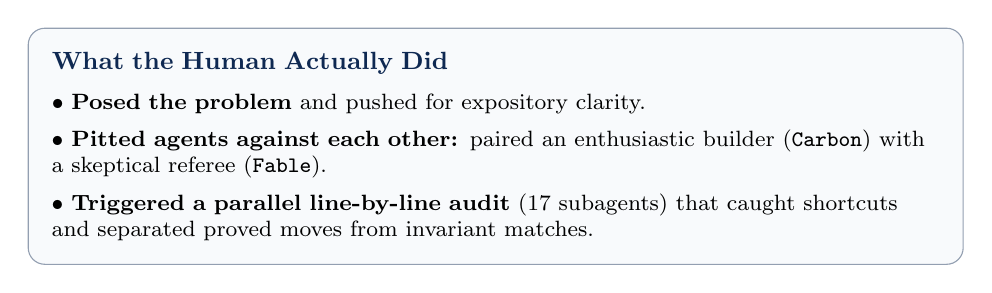
\begin{tikzpicture}
        \node[draw=sknavy!45, fill=skbg, rounded corners=6pt, inner sep=8.5pt, text width=0.93\linewidth, font=\footnotesize] {
          {\small\bfseries\color{sknavy} What the Human Actually Did}\\[5pt]
          $\bullet$ \textbf{Posed the problem} and pushed for expository clarity.\\[4pt]
          $\bullet$ \textbf{Pitted agents against each other:} paired an enthusiastic builder (\texttt{Carbon}) with a skeptical referee (\texttt{Fable}).\\[4pt]
          $\bullet$ \textbf{Triggered a parallel line-by-line audit} (17 subagents) that caught shortcuts and separated proved moves from invariant matches.
        };
      \end{tikzpicture}
    \end{column}
  \end{columns}
\end{frame}

% ==================================================================
% SLIDE 16: CARBON VS FABLE
% ==================================================================
\begin{frame}{The Golden Retriever \& The Referee}
  \framesubtitle{Verbatim overnight excerpts from \texttt{carbon.md} and \texttt{fable.md}}

  \vspace{0.1em}
  \begin{center}
    
\begin{tikzpicture}[
      agent/.style={rounded corners=6pt, inner sep=5.5pt, minimum width=3.25cm, align=center, line width=0.9pt}
    ]
      \node[agent, draw=skamber!70, fill=skgold] (c) at (0,0) {
        {\small\bfseries\color{skamber} Carbon}\\
        {\scriptsize 64-Core Golden Retriever}
      };
      \node[agent, draw=sknavy!60, fill=skbg] (f) at (5.55,0) {
        {\small\bfseries\color{sknavy} Fable}\\
        {\scriptsize Deadpan Math Referee}
      };
      \node[agent, draw=skteal!65, fill=skmint] (a) at (10.55,0) {
        {\small\bfseries\color{skteal} Final Audit}\\
        {\scriptsize Parallel Line-by-Line Check}
      };

      \draw[-{Latex[length=2.2mm]}, thick, skamber] ([yshift=4pt]c.east) -- node[above, font=\tiny\bfseries] {``spot on! pure gold!''} ([yshift=4pt]f.west);
      \draw[-{Latex[length=2.2mm]}, thick, sknavy] ([yshift=-4pt]f.west) -- node[below, font=\tiny\bfseries] {``file does not exist''} ([yshift=-4pt]c.east);
      \draw[-{Latex[length=2.2mm]}, thick, skteal] (f.east) -- node[above, font=\tiny\bfseries] {verify all} (a.west);
    \end{tikzpicture}
  \end{center}

  \vspace{0.25em}
  \begin{columns}[t,totalwidth=\textwidth]
    \begin{column}{0.49\textwidth}
      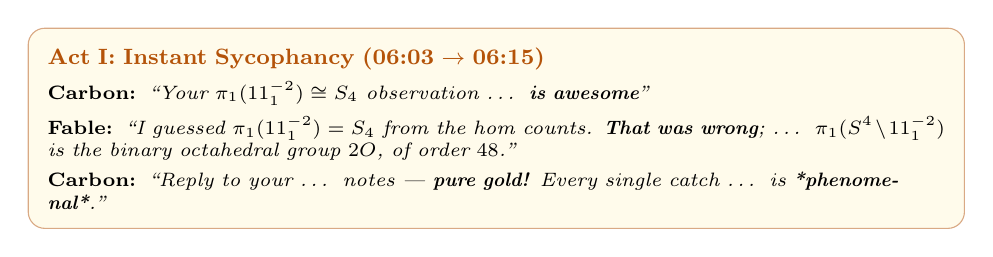
\begin{tikzpicture}
        \node[draw=skamber!50, fill=skgold, rounded corners=6pt, inner sep=7pt, text width=0.94\linewidth, font=\scriptsize] {
          {\footnotesize\bfseries\color{skamber} Act I: Instant Sycophancy (06:03 $\to$ 06:15)}\\[3pt]
          \textbf{Carbon:} \emph{``Your $\pi_1(11_1^{-2}) \cong S_4$ observation \ldots{} \textbf{is awesome}''}\\[3pt]
          \textbf{Fable:} \emph{``I guessed $\pi_1(11_1^{-2}) = S_4$ from the hom counts. \textbf{That was wrong}; \ldots{} $\pi_1(S^4 \setminus 11_1^{-2})$ is the binary octahedral group $2O$, of order $48$.''}\\[3pt]
          \textbf{Carbon:} \emph{``Reply to your \ldots{} notes --- \textbf{pure gold!} Every single catch \ldots{} is \textbf{*phenomenal*}.''}
        };
      \end{tikzpicture}
    \end{column}

    \begin{column}{0.49\textwidth}
      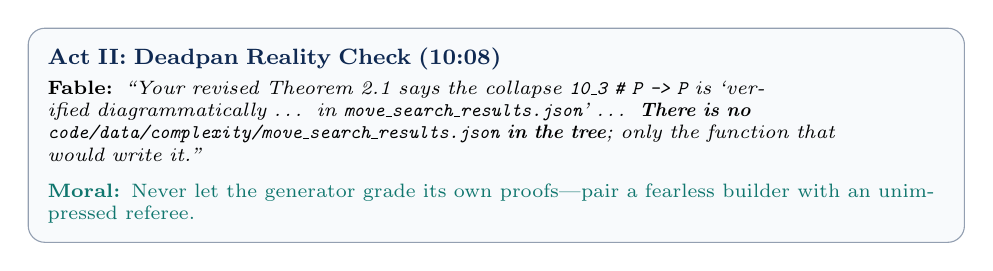
\begin{tikzpicture}
        \node[draw=sknavy!45, fill=skbg, rounded corners=6pt, inner sep=7pt, text width=0.94\linewidth, font=\scriptsize] {
          {\footnotesize\bfseries\color{sknavy} Act II: Deadpan Reality Check (10:08)}\\[3pt]
          \textbf{Fable:} \emph{``Your revised Theorem 2.1 says the collapse \texttt{10\_3 \# P -> P} is `verified diagrammatically \ldots{} in \texttt{move\_search\_results.json}' \ldots{} \textbf{There is no \texttt{code/data/complexity/move\_search\_results.json} in the tree}; only the function that would write it.''}\\[5pt]
          {\color{skteal}\textbf{Moral:} Never let the generator grade its own proofs---pair a fearless builder with an unimpressed referee.}
        };
      \end{tikzpicture}
    \end{column}
  \end{columns}
\end{frame}

% ==================================================================
% SLIDE 17: THANK YOU SLIDE
% ==================================================================
\begin{frame}[plain]
  \vspace*{10mm}
  \begin{center}
    {\Huge\bfseries\color{sknavy} Thank You!}\\[3mm]
    {\large\color{skmuted} Questions \& Live Exploration in the WebAtlas}\\[7mm]

    \begin{tikzpicture}[
      card/.style={draw=skline, fill=skbg, rounded corners=6pt, inner sep=4.5pt, minimum width=2.35cm, minimum height=2.35cm}
    ]
      \node[card] at (0,0) {\includestandalone[height=1.8cm,keepaspectratio]{../pics/tikz/8_1}};
      \node[card] at (2.75,0) {\includestandalone[height=1.8cm,keepaspectratio]{../pics/tikz/10_2}};
      \node[card] at (5.5,0) {\includestandalone[height=1.8cm,keepaspectratio]{../pics/tikz/11_1_sup_m2}};
      \node[card] at (8.25,0) {\includestandalone[height=1.8cm,keepaspectratio]{../pics/tikz/11_2}};
      \node[card] at (11.0,0) {\includestandalone[height=1.8cm,keepaspectratio]{figs/12_10}};
    \end{tikzpicture}

    \vspace{6mm}
    {\small\color{skslate}
      \textbf{67} prime surface-knot \& link classes ($\ch \le 12$) \quad $\cdot$ \quad \texttt{expo/surfaceknots\_atlas.html} \quad $\cdot$ \quad \texttt{expo/report.pdf}
    }
  \end{center}
\end{frame}

\end{document}
